\chapter{Paxos}

In this chapter we provide some background for Paxos and MultiPaxos algorithm. We start with introduction to Paxos and MultiPaxos protocol. Then we describe the problems we encounter while implementing them and performance improvements we made.

\section{Overview}
Paxos algorithm is used to solve consensus problem in distributed system. $n$ processes tries to decide upon the same value, which was proposed by one of them. Paxos does not need a coordinator, however a processes may consider himself a leader for a certain time for specific ballot. As long as there is one leader and the majority of the processes are correct, liveness is guatanteed.

In order to simplify the Paxos as well as for increased preformance, MultiPaxos improvements proposed in \cite{Lam01} introduces one leader for all ballots.

The phase of electing the leader is described in following section. When the leader is elected, it starts proposing new values from clients.

\section{Leader Election}
\label{sec:leader_election}
\indent\par

To decide who is the current leader, our algorithm is using $view$ number. This number is sent in every message and processes keep track of the highest $view$ received. The current leader is a process for which $view \mod n = local~id$. For example, if $view = 5$ and we have $n = 3$ processes then processes with $local~id = 2$ is a current leader.

To detect if a leader is correct, failure detector is used. In JPaxos this is done using heartbeats sent periodically by the leader to all processes. The heartbeats are sent only when there are no other messages being sent, that is, the leader sends an \alive message to the replicas if it didn't sent any message during the last $\tau_0$ time.

When a replica does not receive a message from the leader for more than $\tau_1$ time, it suspects the leader and tries to become the new leader. This phase is called \textbf{prepare phase}. Process advances to the next view where it is the leader and sends a \prepare message to all. For example, if $view = 5$, $n = 3$ and we are process with $local\_id = 1$, we will advance $view$ to number 7 -- first view where process 1 is a leader.

To become a leader, process needs to prepare the view. It sends the \prepare message to all processes with it's new $view$. Every process which received this message, advances its $view$ and responds with \prepareOK. When a process receives majority of \prepareOK message, it becomes a leader. Each \prepareOK message is a promise that the sender will drop all messages with lower view -- that means from old leaders or processes which do not know about the new leader.

\section{Propose Phase}

Every process keeps track of already proposed as well as decided values in a log. A log is ordered list of consensus instances - triple $<id, view, value>$. When a process is a leader, it can start a propose phase for new value. To propose a value, leader creates new consensus instance with first available id, current view and value to propose. Then it is send to all processes in \propose message. Every process when receives the \propose message, saves it to local log and sends \accept message to all. When any process receives the majority of \accept message, it marks the proposed message as decided. The value is then passed to upper layers, in JPaxos executed on the state machine.

\section{Division of responsibility}

As introduced in \cite{Lam01}, the Paxos protocol tasks can eaisly be divided into three groups:
\begin{description}
 \item[Proposer] is responsible for proposing the values in correct order. In JPaxos it takes the requests from Replica and proposes them.
 
 \item[Acceptor] is a part of JPaxos that receives the \propose messages and responds to them according to the Paxos protocol -- that means responds if the view is not lower than current view.
 
 \item[Learner] gathers the \accept messages and if it gets the response from majority of acceptors, it marks them as decided. In JPaxos, it informs the Replica that a decision has been taken.
\end{description}

Our implementation also uses this division in order to make the code more readable. Every process acts as acceptor and learner, and the leader also as proposer.

\section{Concurrent instances}
\label{subsec:concurrent_instances}
Running multiple consensus instances simultaneously is an easy way of making the MultiPaxos algorithm faster. Usually, single instance at time is not able to use available bandwidth; running more makes it possible to use the network more efficiently.

Theoretically, we may have any number of concurrent instances active at the same time. We can execute some decision only after all decisions from all instances with lower number have been executed.

In practical approach, the number of instances must be bounded due to following reasons:
\begin{itemize} 
  \item after leader change, \prepareOK must contain all leader's undecided instances,
  \item network has limited bandwidth, and conducting more instances will not increase throughput,
  \item there is no gain if we have decisions for some future instances, but the decision for an instance with lowest ID has not been taken yet (we can neither respond to the client, nor execute the taken decisions),
  \item using UDP, more concurrent instances are causing network congestion so packets are dropped by the system and instances are decided slower.
\end{itemize}

Biggest problem connected with concurrent instances is possibility of ordering the same request twice. Example scenarios explaining the problem:
\begin{figure*}[ht]
  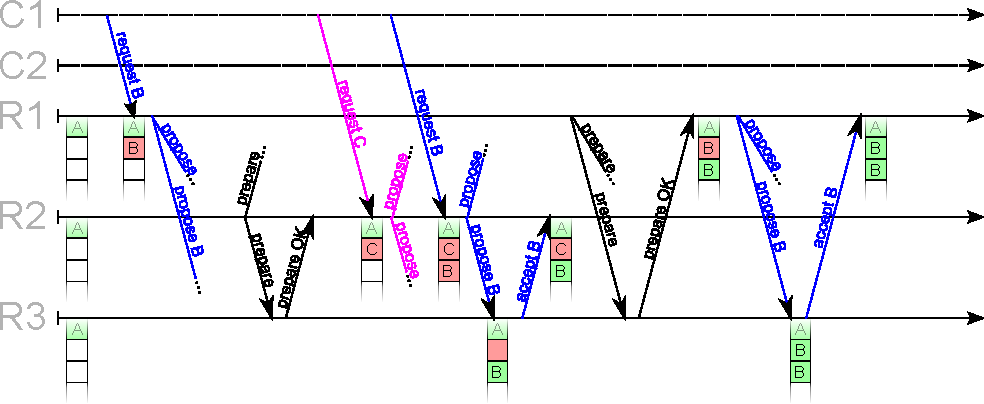
\includegraphics[keepaspectratio, width=\textwidth]{paxos/duplicating_messages.pdf}
  \caption{Duplicating messages - Scenario 1}
\end{figure*}
\begin{description}
  \item [Scenario 1] $R_1$ is the leader, proposes (1:B). No other processes receives these messages and $R_2$ becomes the leader. $R_2$ proposes (1:C) and (2:B). (2:B) is decided. $R_2$ fails and $R_1$ becomes the leader again. While preparing, it learns about (2:B). It has (1:B) as a previously accepted value. The Paxos algorithm requires $R_1$ to propose (1:B) again, since its the accepted value with the highest timestamp, but this will result in the request being decided twice.

  \item [Scenario 2] After a view change, the new primary will know about any value that might have been decided on a previous instance but it might not know about values that were proposed, accepted by up to a minority of replicas but not decided. Suppose that in instance $i$, process $p_1$ had proposed request $R_1$ which was accepted by a minority of replicas. The new primary, $p_2$ doesn't learn about request $R_1$ so it proposes no-op for instance $i$. More or less at the same time, the client resends the request $R_1$ to the new primary, which proposes it and gets it accepted as instance $i+2$, before the no-op request for instance $i$ being accepted. Process $p_2$ crashes and $p_1$ takes over again. Since $p_2$ didn't manage to get no-op accepted for instance $i$, $p_1$ proposes $R_1$ again which ends up being ordered both as instance $i$ and $i+2$.
\end{description} 

Unfortunately we cannot prevent instances from being decided twice in two different instances. Because of that, only valid solution for this problem is to remember last executed instance for every client and not executing them second time. But this requires to keep a new structure in memory as well as by every snapshot (after recovering from snapshot, this structure has to be loaded too).

Even if we cannot prevent from deciding request twice, we should minimise number of such situations because they slow down the algorithm (we have to send redundant data in each message). Possible solutions to decrease them are listed below:
\begin{itemize}
  \item We can cache last reply for each client, so after receiving the same request we can immediately response.
  \item Do not propose requests which are already decided (they can be discarded when creating new batching to propose). 
  \item Current leader can save which requested was proposed by him (but not decided yet) and also discard them. Because in \prepareOK message we can receive instance values which was unknown, leader has to deserialize them first.
\end{itemize}

\paragraph{Setting the window size}
The windows size specifies how many concurrent instances can be started (it has very similar meaning to window size in TCP protocol). In order to use available resources and keep high responsiveness window size must be set correctly. There is no global, generic solution: every usage needs different setting.

Most important thing is monitoring the network: its usage should be high - but no congestion should occur.
That means, on one side, the window size must be enlarged as long as the links are not full, as on the other side, it must be guaranteed that no message will be delayed or dropped because of network traffic.

As long as these conditions hold, a speed of a single instance remains constant (putting aside CPU time).

If network is overused, the overall throughput may even stay on the same level, but the latency will increase for sure.

Notice that having future decisions instead of the present ones does not change decision count per time period, but causes inefficient task arrival time for state machine, especially if many of them arrive at the same time.

\paragraph{Performance Gains}
Single instance will nearly never use available bandwidth, so conducting concurrent instances will surely speed up JPaxos.

In full-duplex networks, concurrent instances will improve network utilisation, because when the leader is waiting for replies, the network from the leader to the followers is idle, so it can be used to send the next request. 

As already mentioned, this solution will improve latency and throughput. Carefulness is required in order to avoid network saturation, especially the link of the leader which has to carry $2n$ messages for each instance (as opposed to 2 messages for every other link).

\paragraph{Batching} is another method for improving performance and network usage. It is preferred over incereasing the concurrent instances count, however the benchmarks show that joining these two methods is better than any of them alone. Batching is described in section \ref{sec:batching}, as it does not concern the Paxos protocol, but values passed to the Proposer.

\section{No operation command}

The best method to understand the problem is to analize the scenario below:

We have three replicas $R1$, $R2$ and $R3$. Replica $R1$ is the leader and proposes {1:A} and {2:B}. Value {2:B} was decided by all replicas, but {1:A} propose was lost. $R1$ fails and $R2$ becomes new leader. After preparing $R2$ has a gap in log because no information about instance 1 was received. 

As we can see after prepare phase, leader can have a gap in the log. Without filling this gap, replica cannot execute and propose new values. Because of that new value has to be proposed in this place.

With crash-stop or crash-recovery without stable storage the value may be lost forever. That happens when decision $n+1$ is already decided, and decision $n$ is unknown to all but leader, and the leader fails. As only he got the value, and it has been lost -- either because he is not allowed to recover, or he is recovering without stable storage.

On the other hand, the leader change may happen due to lost \alive message. In this case someone has the value, and it could be used back in the voting. But there is no simple and fast method to detect this situation.

The easiest solution is to create new request type called no-op, which is null operation and will be ignored by the replica. It fills the gaps, but is not executed on state machine.

\section{Log handling}

The replicated log cannot be allowed to grow forever, it must be bounded in any practical system. After a replica executes some command, it no longer needs the corresponding log entry locally. But other replicas may not have learnt the decision yet. In this case, these late replicas need to learn the decision by asking the corresponding log entry from a replica that still has it.

In JPaxos the Paxos protocol is not used for getting lost requests -- from performance reasons we use the process called ``catch-up'', which is described in section \ref{sec:catch_up}.

So having the old log is needed for view change and, in the crash-recovery model, for recovery.

Especially the latter is problematic. The view change requires always bounded number of instances in log. But if we assume recovery with minimal or no stable storage (as the Epoch based or View based ones), after the recovery a replica needs to recover the state from scratch. For this, it needs whole log -- or the state itself.

\paragraphNewline{Global Commit Point}

A command can be deleted from the log after being executed by all replicas in Crash-stop and Crash-recovery with stable storage models. The highest instance executed by all replicas is called \emph{global commit point}.

But the rule above is not enough to ensure that the log is kept bounded, because a correct replica may be disconnected from the system for some time. When communication is reestablished, the replica needs to learn about all the decisions taken in the meantime. If one replica crashes, the other replicas have no way of knowing that it is a crash and not a disconnection, so they would have to keep the logs forever. And the replica can stay crashed for arbitrarily long time.

Therefore using snapshotting is the only acceptable solution in JPaxos.

\paragraphNewline{Snapshotting}

In order to be able to remove stale log entries, snapshotting should be implemented. It also speeds up the recovery and filling missing instances.

Upon reaching the limit of the log, new snapshot with full state is created and the old logs are truncated even if some other replica doesn't have them yet. When a replica that is missing old logs rejoins, most recent snapshot is transferred first, later all the decisions from the top of the log that were not yet applied to the state.

The size of snapshot is bounded, as the state machine must be implemented with the assumption of bounded memory, and the snapshot may be just the processes memory image. The size of the log is bounded as well -- we create new snapshot as log size reaches some limit.

The problematic part here is the Service -- if the JPaxos library user will not implement creating snapshots or will nor provide them often enough, the log will grow forever.

Snapshotting is described in details in the section \ref{sec:snapshotting}.

\section{Skipping redundant messages}
Reducing number of messages is one of the most efficient optimisation. In JPaxos we do not send messages to self, also the proposer doesn't send \accept messages.

It has been proven for Paxos consensus algorithm that it minimises the count of messages carrying value (client request in our case). The value is sent only once to each replica (not counting retransmission due to message loss). As for additional messages, their count varies among the certain implementations. Some of messages proposed in the typical implementation may be easily skipped without violating guarantees or adding assumptions.

\paragraphNewline{Sending to self}

As stated before, the Paxos can be divided into Proposer, Acceptors and Learners. Processes or some of their parts act as one of them. In order to communicate they must send messages to each other.

In our program every node consists of a (probable) proposer, acceptor as well as learner. In this case there is no need to send messages to self. Especially all send-to-all commands may be replaced by send to others command, as long as the communication with self will be done internally. This skips one \accept and one \propose sent by the leader, and one \accept by all other processes.

This does not influence the performance much, however it is recommended as it decreases system -- especially networking stack -- usage. It also skips a few system calls.

\paragraphNewline{Using {\normalfont\propose}as {\normalfont\accept}}

More important optimisation is merging the role of \accept and \textsc{Propose}. As long as acceptors and proposes do not share the log this is not allowed. But if their knowledge is identical and the leader proposed some value, then he must accept it as well. In most solutions one node acts as proposer and acceptor, and they do share the log.

So in JPaxos each \propose is simultaneously an \accept message. Notice that if the system consists of three nodes every process decides on the value by receiving a valid propose -- he knows that the leader and he himself accept the message. Normally the leader process has to send \propose to all first, later \accept to all. By this optimisation we are required to send the half of messages only.

This is a serious gain, clearly visible during benchmarks.

\paragraphNewline{Minimizing messages with value}

Most of the articles about Paxos state that the \accept message carries the value. This can be easily omitted.

Each processes in JPaxos waits not only for the majority of accepts, but before it sends the \accept message, it must receive a \propose with the value. So if a process accepts an instance, it already knows the value.

Waiting for another message might seem to cause additional overhead, but it makes JPaxos faster -- less network bandwidth is used by a single instance. Also ususally the \propose will be delivered before any \accept message.

\paragraphNewline{Best-case messages}
\label{par:bestCaseMessages}

So, in normal operation in JPaxos:

\begin{tabular}{llllll}
          & Processes & Count & Time & Message  & Value  \\
 Proposer & $1$       & $n$   & $n$  & \propose & yes    \\
 Acceptor & $n-1$     & $n-1$ & 1    & \accept  & no
\end{tabular}

We can see that in order to decide we need to send once the \propose, and later each not-leader process sends the \accept to others.

Other implementations consider using bounded learner count -- so that a acceptor sends \accept only to them. An additional message, \textsc{Decided}, is sent by Learners to all as the ballot nas finished. Thanks to this modification no reliable broadcast is needed, but also an additional phase must occur.

Interesting approach is presented in the RingPaxos (see \cite{Mar10}), where IP multicast is used for all broadcasts, what masively increases the scalability and performance.
